\section{Question 2: Named Entity Recognition}

\subsection{Dataset Description}

Question 2 uses the English CoNLL-2003 named entity recognition benchmark \cite{tjong2003conll} with the IOB2 tagging scheme and four entity types: PER, ORG, LOC, and MISC. The local environment could not load the legacy script-based dataset entry directly, so the experiments used the Hugging Face mirror \texttt{tomaarsen/conll2003}, which preserves the same token-level label inventory. The final split sizes were 14{,}041 training sentences, 3{,}250 validation sentences, and 3{,}453 test sentences. Model selection focused on strict entity-level precision, recall, and F1 under the IOB2 scheme, while token accuracy was retained as a supplementary diagnostic metric.

\subsection{Preprocessing and BIO Alignment}

All models consume the original tokenized sentence boundaries from CoNLL-2003. For the feature-based CRF, each token is represented by local orthographic and contextual cues including the lowercased token form, short prefixes and suffixes, case indicators, digit and hyphen flags, token length, and previous or next token features with beginning-of-sequence and end-of-sequence markers. The BiLSTM-CRF model operates on word-level token ids with padding and masking so that sequence length is preserved during recurrent encoding and CRF decoding.

The BERT model uses \texttt{bert-base-cased} because capitalization is informative for named entities. Word-level gold tags are aligned to subword tokenization by assigning the original tag only to the first subword of a word and setting special tokens or continuation subwords to \texttt{-100}, which removes them from the loss. This keeps optimization aligned with word-level evaluation while still allowing the model to benefit from subword segmentation.

\subsection{Models}

\paragraph{Feature CRF.}
The classical baseline is a linear-chain CRF \cite{lafferty2001crf} trained with the \texttt{lbfgs} optimizer, \(c_1 = 0.1\), \(c_2 = 0.1\), 100 maximum iterations, and all transitions enabled. This model relies entirely on the engineered token and context features described above.

\paragraph{BiLSTM-CRF.}
The hybrid neural baseline uses 100-dimensional token embeddings, a single bidirectional LSTM layer with hidden size 128, dropout 0.3, batch size 32, and AdamW optimization with learning rate 0.001. The model was trained for up to eight epochs with early stopping on validation F1. The CRF output layer preserves global transition constraints during decoding.

\paragraph{BERT Token Classification.}
The transformer baseline fine-tunes \nolinkurl{bert-base-cased} \cite{devlin2019bert} with maximum sequence length 128, batch size 8, learning rate \(5 \times 10^{-5}\), weight decay 0.01, warmup ratio 0.1, and early stopping patience 2. The strongest full-data run completed after two epochs and clearly outperformed the non-transformer baselines.

\subsection{Results}

Table~\ref{tab:q2_overall_results} summarizes the overall validation and test metrics. BERT produced the strongest result by a wide margin, reaching test F1 0.9062. The feature-based CRF remained a strong non-transformer baseline at test F1 0.7948. BiLSTM-CRF improved over its smoke-test behavior but still lagged behind both alternatives at test F1 0.7145.

\begin{table}[H]
\centering
\small
\begin{tabular}{lccccccc}
\toprule
Model & Val. P & Val. R & Val. F1 & Test P & Test R & Test F1 & Test Acc. \\
\midrule
BERT & 0.9525 & 0.9509 & 0.9517 & 0.9028 & 0.9095 & 0.9062 & 0.9807 \\
Feature CRF & 0.8939 & 0.8596 & 0.8765 & 0.8131 & 0.7773 & 0.7948 & 0.9572 \\
BiLSTM-CRF & 0.8292 & 0.7625 & 0.7945 & 0.7674 & 0.6684 & 0.7145 & 0.9373 \\
\bottomrule
\end{tabular}
\caption{Overall Q2 NER performance on the validation and test splits.}
\label{tab:q2_overall_results}
\end{table}

Table~\ref{tab:q2_per_entity_results} breaks the test results down by entity type. The support column corresponds to the number of gold entities in the test set. BERT dominates every entity category, with especially strong performance on PER and LOC. MISC is the hardest category for all models and remains the main source of residual error even in the strongest system.

\begin{table}[H]
\centering
\small
\begin{tabular}{llcccc}
\toprule
Model & Entity & Precision & Recall & F1 & Support \\
\midrule
BERT & LOC & 0.9269 & 0.9269 & 0.9269 & 1668 \\
Feature CRF & LOC & 0.8442 & 0.8249 & 0.8344 & 1668 \\
BiLSTM-CRF & LOC & 0.7991 & 0.7680 & 0.7832 & 1668 \\
\midrule
BERT & MISC & 0.7693 & 0.8077 & 0.7880 & 702 \\
Feature CRF & MISC & 0.7756 & 0.7436 & 0.7593 & 702 \\
BiLSTM-CRF & MISC & 0.7157 & 0.6239 & 0.6667 & 702 \\
\midrule
BERT & ORG & 0.8873 & 0.8958 & 0.8916 & 1661 \\
Feature CRF & ORG & 0.7711 & 0.6773 & 0.7212 & 1661 \\
BiLSTM-CRF & ORG & 0.7359 & 0.6273 & 0.6773 & 1661 \\
\midrule
BERT & PER & 0.9552 & 0.9499 & 0.9526 & 1617 \\
Feature CRF & PER & 0.8351 & 0.8454 & 0.8402 & 1617 \\
BiLSTM-CRF & PER & 0.7873 & 0.6271 & 0.6981 & 1617 \\
\bottomrule
\end{tabular}
\caption{Per-entity test metrics for the completed Q2 runs.}
\label{tab:q2_per_entity_results}
\end{table}

Figure~\ref{fig:q2_entity_f1} visualizes the per-entity test F1 comparison. The same pattern is visible across all entity types: contextualized BERT representations yield the best scores, CRF remains competitive without pretrained embeddings, and the recurrent hybrid model underperforms despite having a structured decoder.

\begin{figure}[H]
    \centering
    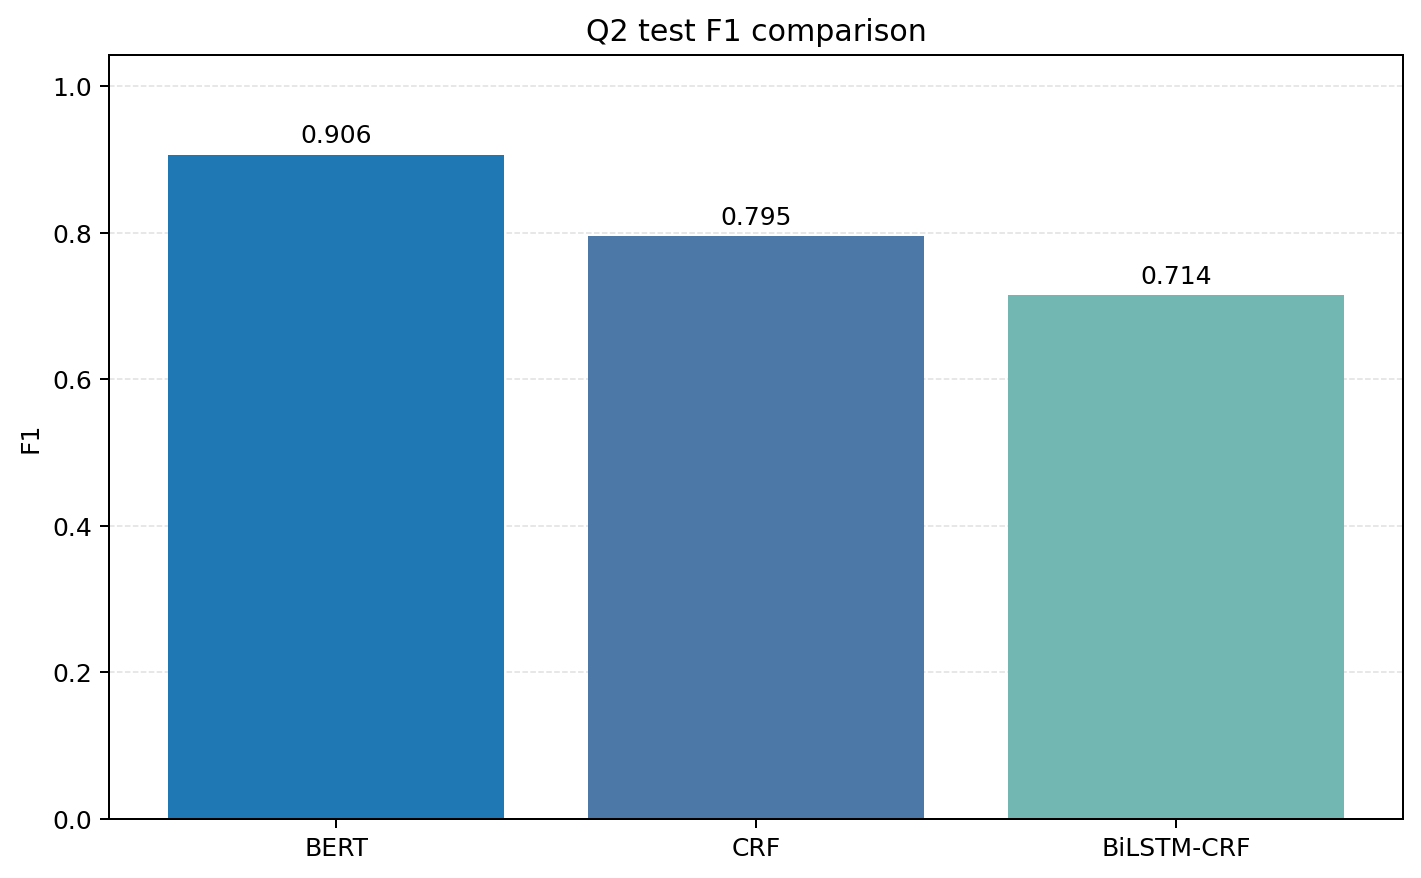
\includegraphics[width=0.85\textwidth]{figures/q2/entity_f1_comparison.png}
    \caption{Per-entity test F1 comparison for the completed Q2 CRF, BiLSTM-CRF, and BERT runs.}
    \label{fig:q2_entity_f1}
\end{figure}

\subsection{Error Analysis}

The exported error-analysis artifacts show qualitatively different failure modes across the three models. For the feature CRF, the most common test confusion is \texttt{B-ORG \(\rightarrow\) O}, which indicates missed organization boundaries and weaker recall on organization names. BiLSTM-CRF fails most often on person entities, with \texttt{B-PER \(\rightarrow\) O} as its dominant confusion; this is consistent with its lower recall and suggests that the recurrent encoder did not exploit enough context to recover entity starts reliably. BERT still makes mistakes, but its main confusion pattern is \texttt{O \(\rightarrow\) I-MISC}; in practice this means that the model occasionally overextends rare miscellaneous entities while still preserving much stronger overall entity recall and boundary quality than the alternatives.

The per-entity table supports this interpretation. Under BERT, MISC remains the weakest class at F1 0.7880, whereas PER and LOC both exceed 0.92 F1. This suggests that contextual embeddings largely solve boundary and lexical ambiguity for common entity categories, while rarer and semantically broader labels such as MISC still require additional disambiguation.

\subsection{Discussion}

The final ranking for Question 2 is clear: BERT is the strongest model, the feature-based CRF is the strongest non-transformer baseline, and BiLSTM-CRF is the weakest of the completed full-data runs. This outcome highlights two practical points. First, pretrained contextual representations are substantially more valuable than either engineered local features or a randomly initialized recurrent encoder on this task. Second, a well-configured classical CRF can still outperform a neural hybrid model when the latter is not tuned enough to convert representation power into better sequence decisions.

From a report perspective, the BERT run should anchor the main Q2 claim, while the CRF result should be presented as a surprisingly strong and interpretable baseline. BiLSTM-CRF is still useful as a comparison point because it demonstrates that adding recurrence and a CRF layer alone is not sufficient to close the gap to transformer-based contextualization. If additional Q2 effort becomes available later, the most justified follow-up is a focused BiLSTM-CRF tuning slice or a deeper MISC-specific error analysis rather than another baseline implementation.